\documentclass[a4paper, 14pt]{extarticle}%тип документа

%Русский язык
\usepackage[T2A]{fontenc} %кодировка
\usepackage[utf8]{inputenc} %кодировка исходного кода
\usepackage[english,russian]{babel} %локализация и переносы

%отступы 
\usepackage[left=2cm,right=2cm,top=2cm,bottom=3cm,bindingoffset=0cm]{geometry}

%Вставка картинок
\usepackage{graphicx}
\usepackage{wrapfig, caption}
\graphicspath{}
\DeclareGraphicsExtensions{.pdf,.png,.jpg, .jpeg}
\newcommand\ECaption[1]{%
     \captionsetup{font=footnotesize}%
     \caption{#1}}

%Таблицы
\usepackage[table,xcdraw]{xcolor}
\usepackage{booktabs}

%Графики
\usepackage{pgfplots}
\pgfplotsset{compat=1.9}

%Математика
\usepackage{amsmath, amsfonts, amssymb, amsthm, mathtools}

%Заголовок
\author{Подлесный Артём \\ группа 827}
\title{Работа 10.1 \\ Электронный парамагнитный резонанс}

\begin{document}
\maketitle

\section*{Краткая теория}

\begin{figure}[h]
\begin{center}
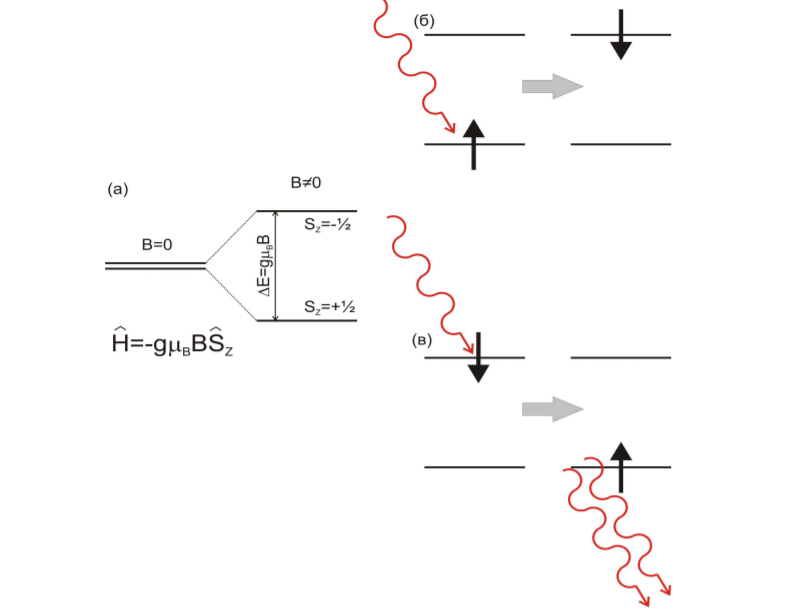
\includegraphics[width=0.6\textwidth]{teor}
\end{center}
\ECaption{Схема резонансного поглощения электромагнитного излучения для изолированного
спина $S=1/2$. (a) Зеемановское расщепление спинового уровня в магнитном поле. (б) Переход
между подуровнями снизу-вверх с поглощением фотона резонансной частоты
$h \nu=g \mu_B B $. (в) Переход между подуровнями сверху-вниз с излучением дополнительного
фотона резонансной частоты.}
\end{figure}
В состоянии теплового
равновесия нижний энергетический уровень более заселён, поэтому наблюдается
поглощение электромагнитного излучения. 

Расщепление терма свободного иона по проекции спина определяется $g-$фактором Ланде:
\begin{equation}
E(m_s) = g \mu_B B m_s
\end{equation}
В данном случае расщепление происходит в кристалле, поэтому формулу нужно изменить, введя вместo $g$ эффективный фактор - $g_{\text{эфф}}$. Тогда его можно измерить по следующей формуле:
\begin{equation}
g_{\text{эфф}} = \frac{h\nu}{\mu_B B}.
\end{equation}

\section*{Экспериментальная установка}

\begin{figure}[h!]
\begin{minipage}[h]{0.5\linewidth}
\center{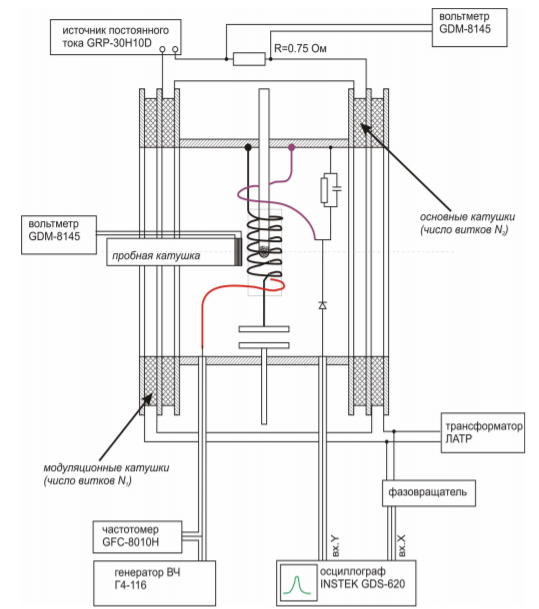
\includegraphics[width=1\linewidth]{ust1} \\ (a)}
\end{minipage}
\hfill
\begin{minipage}[h]{0.5\linewidth}
\center{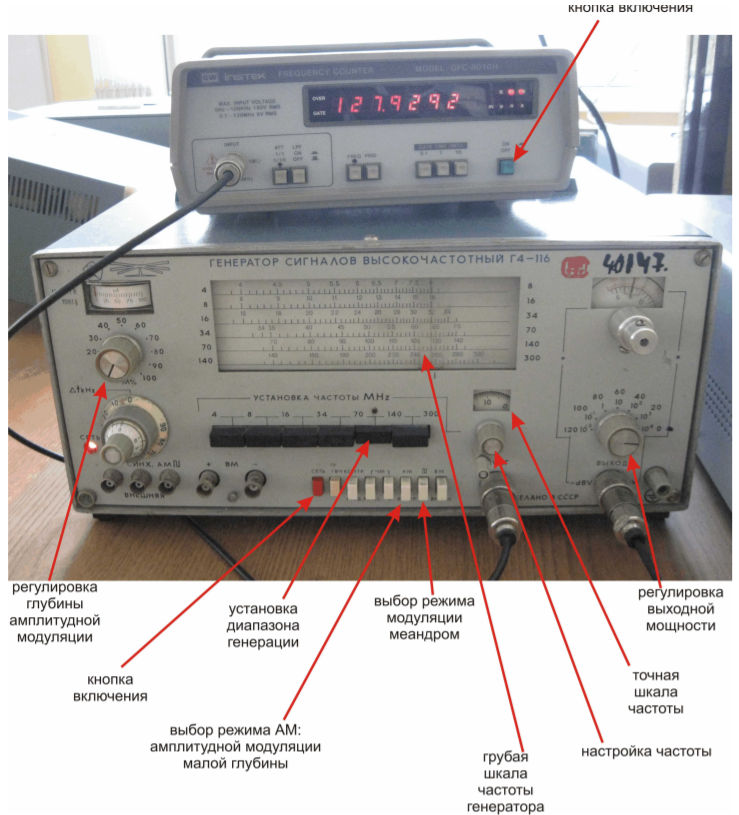
\includegraphics[width=1\linewidth]{ust2} \\ (б)}
\end{minipage}
\ECaption{a) Схема установки для наблюдения электронного парамагнитного резонанса. б) Генератор ВЧ и частотометр.}
\end{figure}

Для проведения эксперимента использовалась установка на рис. 2.
Частотометр обладал ручкой тонкой настройки, однако она не отображала действительные значения десятых долей, а была относительной шкалой. Поэтому результаты измерений резонансных частот были нормированы, использую показания тонкой шкалы на 2 соседних показаниях грубой шкалы.

Параметры установки для дальнейших измерений были известны.


\section*{Наблюдение сигнала ЭПР. Определение g-фактора и ширины линии ЭПР.}

Данный эксперимент включал в себя 2 подготовительных этапа:
\paragraph*{Настройка ВЧ генератора:} необходимо было настроить генератор на резонансную частоту, что наблюдалось как резкое увеличение аплитуды сигнала на осциллографе. Полученное значение частоты резонанса составило:
\[f_0 = 132.45 \text{ }MHz.\]
Тогда, с помощью частот, на которых амплитуда сигнала уменьшается в 2 раза по сравнению с резонансным, можно оценить добротность схемы как:
\[Q = \frac{f_0}{f_{+\frac{1}{2}}-f_{-\frac{1}{2}}} \approx 631.\]

\paragraph*{Наблюдение сигнала резонансного поглощения.}
Основные катушки были подключены  к источнику постоянного тока, а модуляционные катушки к
трансформатору ЛАТР.
\begin{wrapfigure}{r}{0.4\textwidth}
\begin{center}
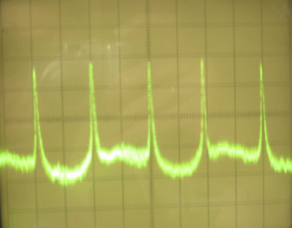
\includegraphics[height=6cm]{ust3}
\end{center}
\ECaption{Осциллограмма сигнала когда постоянное поле
близко к резонансному, пики практически эквидистантны.}
\end{wrapfigure}

Поле на образце является суммой постоянного поля от основных катушек и переменного
поля от модуляционных катушек 
$B(t) = B_{\text{пост}} + B_{\text{мод}}\sin (\omega_{\text{мод}}t)$. Резонансное поглощение наступает при совпадении поля катушек с полем поглощения $B_0 = \frac{hf_0}{\mu_B g_{\text{эфф}}}$ Необходимо настроить поле $B_{\text{пост}}$ на резонансное $B_0$. Тогда на осциллографе буду видны эквидистантные пики, изображенные на рис.3.

\subsection*{Точная настройка резонансного поля и определение ширины линии}

Подав на Х-канал осциллографа напряжение с модуляционных катушек, можно увидеть в режиме Х-Y линию ЭПР. После тонкой настройки, можно получить точную линию ЭПР. изобрвженную на рис. 4.

\begin{figure}[h]
\begin{center}
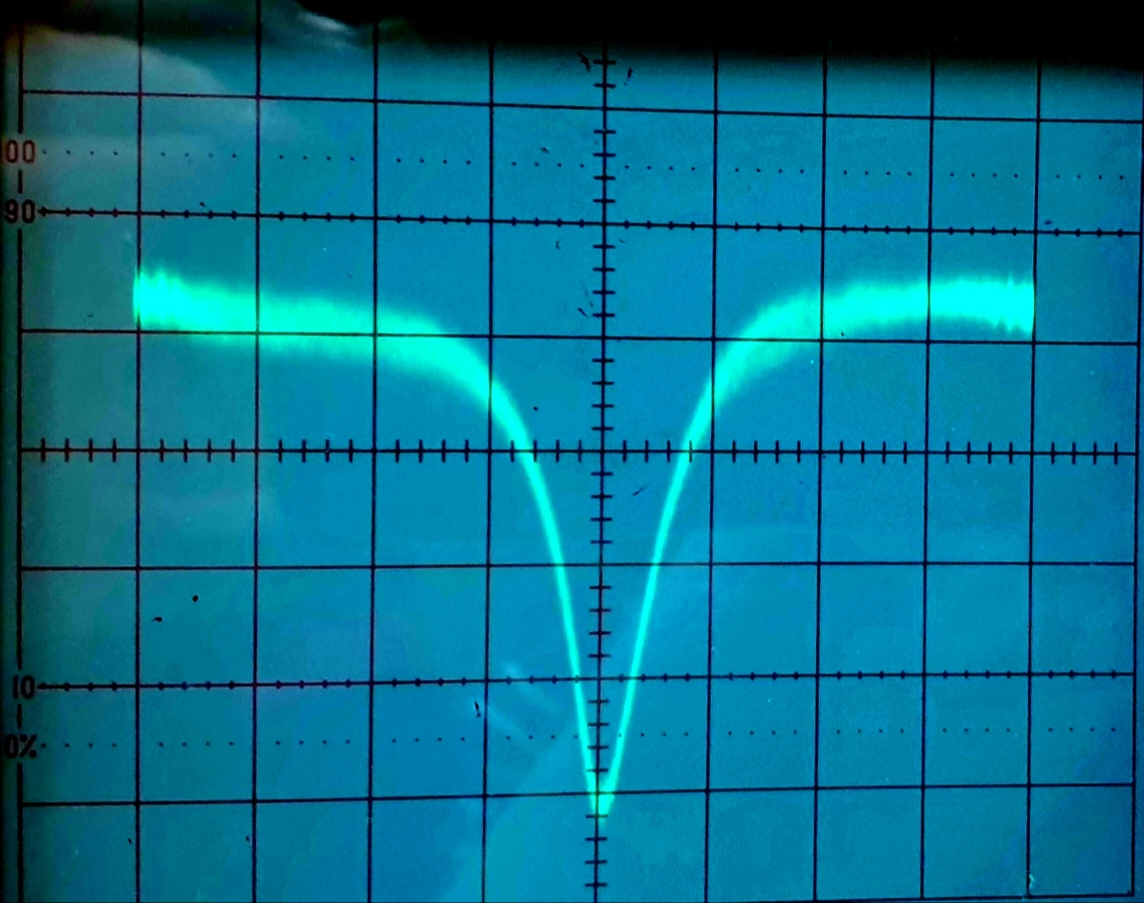
\includegraphics[width=0.6\textwidth]{epr}
\end{center}
\ECaption{Линия поглощения ЭПР в режиме XY-развёртки при практически точной настройке.}
\end{figure}

По полученной картине можно найти  полный размах
модулирующего поля (в делениях шкалы) $A_{\text{полн}} = 40$ и полную ширину кривой резонансного
поглощения на полувысоте $A_{\frac{1}{2}} = 5$. Тогда, внеся внутрь соленоида пробную катушку, можно определить амплитуду модулирующего поля как:
\[B_{\text{мод}} = \sqrt{2} \frac{2\xi}{\pi^2 d^2 N_{\text{пробн}} \nu}   =  0.98\pm0.03 \text{ мТл},\]
где $\xi = 1.61$ -- ЭДС индукции в пробной катушке. 

Полуширина на полувысоте линии резонансного
поглощения (в единицах поля) может быть тогда получена как
\[\Delta B = \frac{A_{\frac{1}{2}}}{A_{\text{полн}}}B_{мод} = 0.12\pm0.02\text{ мТл}.\]
\subsection*{Калибровка поля электромагнита и определение g-фактора}
Чтобы определить связь между падением напряжения на резисторе в цепи основных
катушек и магнитным полем в центре магнита, в соленоид спереди и сзади вносилась пробная катушка. Проводилось несколько калибровочных измерений ЭДС пробной катушки и напряжения на соленоиде. Результаты представлены на таблице.
\begin{table}[h!]
\begin{center}
\begin{tabular}{|c|c|c|}
\hline
\rowcolor[HTML]{6665CD} 
        & cпереди   & cзади     \\ \hline
\rowcolor[HTML]{9698ED} 
$U$, mV & $\xi$, mV & $\xi$, mV \\ \hline
50      & 4.19      & 4.26      \\ \hline
\rowcolor[HTML]{9698ED} 
70      & 5.89      & 5.95      \\ \hline
80      & 6.75      & 6.8       \\ \hline
\rowcolor[HTML]{9698ED} 
100.3   & 8.47      & 8.5       \\ \hline
110.6   & 9.34      & 9.38      \\ \hline
\rowcolor[HTML]{9698ED} 
131     & 11.08     & 11.09     \\ \hline
150.4   & 12.72     & 12.71     \\ \hline
\end{tabular}
\ECaption{Результаты измерения зависимости $U(\xi)$ при поднесении катушки к образцу спереди и сзади установки.}
\end{center}
\end{table}

По полученным данным построен график (рис.5).
\begin{figure}[h]
\begin{center}
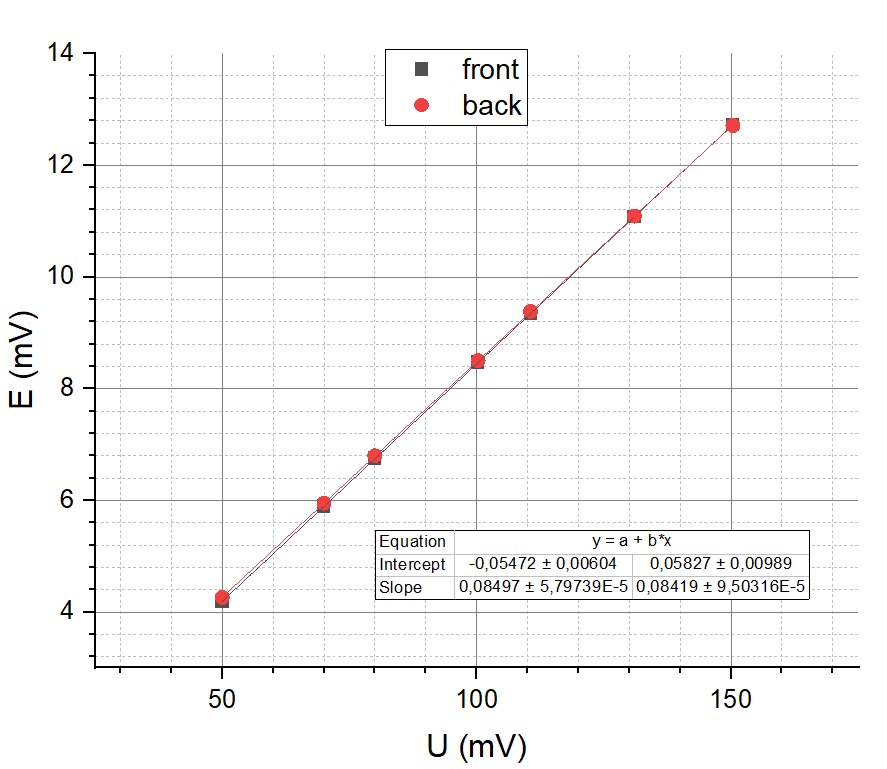
\includegraphics[width=0.9\textwidth]{gr1}
\ECaption{Зависимость ЭДС индукции пробной катушки от напряжения на резисторе основных катушек. На графике нанесены точки, измеренные середи и сзади образца, однако они совпадают, как графически, так и их коэффициенты наклона. Это говорит о хорошей геометрии установки и симметричном распределении поля.}
\end{center}
\end{figure}

Теперь необходимо связать эти данные со значением магнитного поля в образце. Для магнитного потока через пробную катушку получаем:
\begin{equation}
\Phi = B_0 N_{\text{пробн}} \frac{\pi d^2}{4} = \frac{Slope\cdot U \cdot 2\pi}{\nu}
\end{equation}
Тогда для магнитного поля в условиях резонанса получим:
\begin{equation}
B_0 = \frac{4\cdot Slope\cdot U}{\omega \pi N_{\text{пробн}} d^2} = 4.5\pm0.1\text{ мТл}.
\end{equation}

Тогда, используя значение для резонансной частоты получаем результат для $g-$фактора по формуле (2):
\[g_{\text{эфф}} = 2.10\pm 0.14.\]
Результат в описании к лабе составляет $g = 2.0036$ для ДФПГ, так что с учетом погрешности результаты вполне совпадают с действительностью.
\newpage
\section*{Измерение на нескольких частотах}

Измененяя зазор в конденсаторе схемы, можно изменять параметры установки, тогда резонансное напряжение для поглощения будет отличаться. Результаты таких измерений представлены на таблице 2.

\begin{table}[h!]
\begin{center}
\begin{tabular}{|c|c|}
\hline
\rowcolor[HTML]{9698ED} 
$f$, MHz & $U$, mV \\ \hline
135.74   & 134.82  \\ \hline
\rowcolor[HTML]{9698ED} 
88.46    & 88.19   \\ \hline
94.85    & 92.65   \\ \hline
\rowcolor[HTML]{9698ED} 
100.00   & 98.43   \\ \hline
108.00   & 108.06  \\ \hline
\rowcolor[HTML]{9698ED} 
114.00   & 113.85  \\ \hline
120.00   & 119.73  \\ \hline
\rowcolor[HTML]{9698ED} 
125.36   & 124.88  \\ \hline
\end{tabular}
\ECaption{Зависимость резонанстной частоты контура $f(U)$ от напряжения поглощения.}
\end{center}
\end{table}

По этим данным был построен график, изображенный на рис.6.

\begin{figure}[h]
\begin{center}
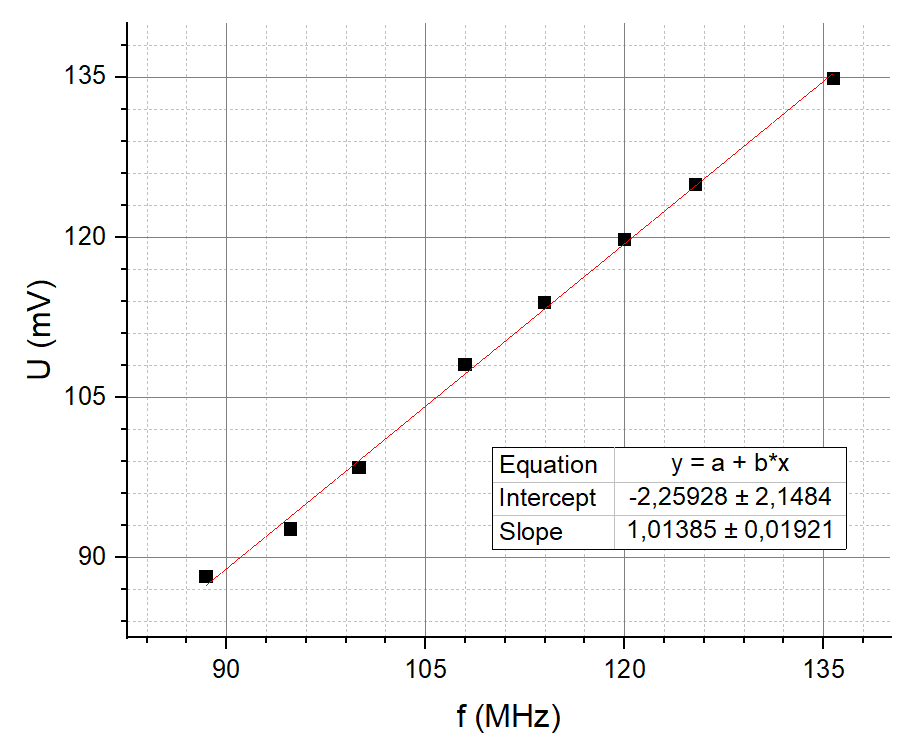
\includegraphics[width=0.9\textwidth]{gr2}
\ECaption{График зависимости резонанстной частоты контура $f(U)$ от напряжения поглощения. Он вполне неплохо аппроксимируется линейной зависимостью.}
\end{center}
\end{figure}

Как видно, график неплохо аппроксимируется линейной зависимостью, что показывает, что в пределах точности эксперимента он соответствует линейному расщеплению спиновых подуровней.

Используя формулу (2), уточняем $g-$фактор:
\[g_{\text{эфф}} = 2.07\pm0.06\]

\newpage

\section*{Вывод}

В работе был измерен $g-$фактор ДФПГ с хорошей точностью, был продемонстрирован электронный парамагнитный резонанс, а так же был подтвержден линейный характер Зеемановского расщепления спиновых подуровней.

\end{document}